% The generic preamble
\documentclass[10pt,letterpaper,fleqn,titlepage]{article}

% Define packages to use
\usepackage{natbib}
\usepackage[dvips]{graphicx,color}
\usepackage{amsmath,amssymb}
\usepackage{bm}
\usepackage{caption}
\usepackage{xr}
\usepackage{ifthen}
\usepackage[dvipdfm,colorlinks,linkcolor=blue,citecolor=blue,urlcolor=blue]{hyperref}
\usepackage{fancybox}
\usepackage{textcomp}
\usepackage{alltt}
%\usepackage{floatflt}
%\usepackage{svn}


% Redefine default page
\setlength{\textheight}{9in}  % 1" above and below
\setlength{\textwidth}{6.75in}   % 0.5" left and right
\setlength{\oddsidemargin}{-0.25in}

% Redefine default paragraph
\setlength{\parindent}{0pt}
\setlength{\parskip}{1ex plus 0.5ex minus 0.2ex}

% Define caption width and default fonts
\setlength{\captionmargin}{0.5in}
\renewcommand{\captionfont}{\sffamily}
\renewcommand{\captionlabelfont}{\bfseries\sffamily}

% Define commands for super- and subscript in text mode
\newcommand{\superscript}[1]{\ensuremath{^\textrm{#1}}}
\newcommand{\subscript}[1]{\ensuremath{_\textrm{#1}}}

% Derived commands
\newcommand{\invcm}{\textrm{cm\superscript{-1}}}
\newcommand{\micron}{\ensuremath{\mu\textrm{m}}}

\newcommand{\df}{\ensuremath{\delta f}}
\newcommand{\Df}{\ensuremath{\Delta f}}
\newcommand{\dx}{\ensuremath{\delta x}}
\newcommand{\Dx}{\ensuremath{X_{max}}}
\newcommand{\Xeff}{\ensuremath{X_{eff}}}

\newcommand{\water}{\textrm{H\subscript{2}O}}
\newcommand{\carbondioxide}{\textrm{CO\subscript{2}}}
\newcommand{\ozone}{\textrm{O\subscript{3}}}

\newcommand{\taup}[1]{\ensuremath{\tau_{#1}}}
\newcommand{\efftaup}[1]{\ensuremath{\tau_{#1}^{*}}}

\newcommand{\textbfm}[1]{\boldmath\ensuremath{#1}\unboldmath}

\newcommand{\rb}[1]{\raisebox{1.5ex}[0pt]{#1}}

\newcommand{\f}[1]{\texttt{#1}}

% Define how equations are numbered
\numberwithin{equation}{section}
\numberwithin{figure}{section}
\numberwithin{table}{section}

% Define a command for title page author email footnote
\newcommand{\email}[1]
{%
  \renewcommand{\thefootnote}{\alph{footnote}}%
  \footnote{#1}
  \renewcommand{\thefootnote}{\arabic{footnote}}
}

% Define a command to print the Office Note subheading
\newcommand{\notesubheading}[1]
{%
  \ifthenelse{\equal{#1}{}}{}
  { {\Large\bfseries Office Note #1\par}%
    {\scriptsize \sc This is an unreviewed manuscript, primarily intended for informal}\\ 
    {\scriptsize \sc exchange of information among JCSDA researchers\par}%
  }
}

% Redefine the maketitle macro
\makeatletter
\def\docseries#1{\def\@docseries{#1}}
\def\docnumber#1{\def\@docnumber{#1}}
\renewcommand{\maketitle}
{%
  \thispagestyle{empty}
  \vspace*{1in}
  \begin{center}%
     \sffamily
     {\huge\bfseries Joint Center for Satellite Data Assimilation\par}%
     \notesubheading{\@docnumber}
  \end{center}
  \begin{flushleft}%
     \sffamily
     \vspace*{0.5in}
     {\Large\bfseries\ifthenelse{\equal{\@docseries}{}}{}{\@docseries: }\@title\par}%
     \medskip
     {\large\@author\par}%
     \medskip
     {\large\@date\par}%
     \bigskip\hrule\vspace*{2pc}%
  \end{flushleft}%
  \newpage
  \setcounter{footnote}{0}
}
\makeatother
\docseries{}
\docnumber{}


% Define a command for a DRAFT watermark
\usepackage{eso-pic}
\newcommand{\draftwatermark}
{
  \AddToShipoutPicture{%
    \definecolor{lightgray}{gray}{.85}
    \setlength{\unitlength}{1in}
    \put(2.5,3.5){%
      \rotatebox{45}{%
        \resizebox{4in}{1in}{%
          \textsf{\textcolor{lightgray}{DRAFT}}
        }
      }
    }
  }
}




% Define included documents
\includeonly{Change_History,Introduction,Repository_Organisation,Build_Conventions,Commit_Log_Messages}

% Generic fixed font command
\newcommand{\f}[1]{\texttt{#1}}
\newcommand{\subversion}{\href{http://subversion.tigris.org/}{subversion}}
\newcommand{\trac}{\href{http://trac.edgewall.org/}{\textsf{trac}}}

% Title info
\title{Subversion Repository and trac SCM Guide}
\author{Paul van Delst\email{paul.vandelst@noaa.gov}\\JCSDA/EMC/SAIC}
\date{August, 2009}


%-------------------------------------------------------------------------------
%                            Ze document begins...
%-------------------------------------------------------------------------------
\begin{document}
\maketitle

% The front matter
%=================
% The Change History table
% ========================
\thispagestyle{empty}
\vspace*{10cm}
\begin{center}
  {\sffamily\Large\bfseries Change History}
  \begin{table}[htp]
    \centering
    \begin{tabular}{|p{2cm}|p{3cm}|p{8cm}|}
      \hline
      \sffamily\textbf{Date} & \sffamily\textbf{Author} & \sffamily\textbf{Change}\\
      \hline\hline
      2008-08-29 & P.van Delst & Initial release.\\
      \hline
      2008-08-30 & P.van Delst & Added Build Conventions chapter.\\
      \hline
      2008-11-06 & P.van Delst & Added Commit Log Messages chapter.\\
                 &             & Added bibliography.\\
      \hline
      2009-08-12 & P.van Delst & Updated for new server URL.\\
                 &             & Updated branching structure description. \\
      \hline
    \end{tabular}
  \end{table}
\end{center}
\clearpage

\setcounter{page}{1}
\pagenumbering{roman}
  \tableofcontents\newpage
  \listoffigures\newpage
  \listoftables\newpage
\pagenumbering{arabic}
\setcounter{page}{1}

% Include all the sections
%=========================
\chapter{Introduction}
%=====================


\section{Components}
%===================
\label{sec:components}

The LBLRTM I/O library is constructed around five data constructs, described in table \ref{tab:component_definitions}:
\begin{table}[htp]
  \centering
  \caption{The data constructs of the LBLRTM I/O library}
  \begin{tabular}{p{2.5cm} p{12cm}}
    \hline\\[-0.1cm]
    \sffamily\textbf{Component Name} & \sffamily\textbf{Description} \\
    \hline\hline\\[-0.2cm]
    \texttt{Fhdr}  & The file header construct that is present at the start of each layer of data. \\\\
    \texttt{Phdr}  & This is the panel header construct that is present at the start of each ``chunk'' of data (usually referred to as a ``panel''. See following.) \\\\
    \texttt{Panel} & This construct corresponds to a ``chunk'' of spectral data. An LBLRTM datafile is referred to as being a single- or double-panel file. The former means a single spectral quantity is present (e.g. optical depth), and the latter means that two spectral quantities are present (e.g. radiance and transmittances). \\\\
    \texttt{Layer} & This construct contains spectral data for the entire frequency range of an LBLRTM calculation for a single layer. The concept ``layer'' can correspond to the spectral data for individual atmospheric layers of the input profile, or to the final result for an entire atmosphere. \\\\
    \texttt{File}  & This contruct is true to its name. It corresponds to an entire datafile of data which may consist of a single layer or multiple layers, and for single- or double-panel spectral data. \\
  \hline
  \end{tabular}
  \label{tab:component_definitions}
\end{table}

Each component has a definition module to define the object and some basic methods to manipulate it, and an I/O module to read and write instances of the objects from/to file.

Two components -- the file header and panel header -- are standalone, but the others contain other components, i.e. the panel object contains panel headers; the layer object contains file headers; and the file object contains layers. A schematic illustration of how the actual LBLRTM datafile format relates to the component definitions is shown in figure \ref{fig:lblrtm_format}.

Note, however, that when an LBLRTM file is read, the individual panel ``chunks'' of spectral data are concatenated into a single spectrum. Thus the \Panel{} object itself is only used when reading from an LBLRTM file and is not used in the \File{} or \Layer{} objects.

\begin{figure}[htp]
  \centering
  \input{graphics/lblrtm_format.pstex_t}
  \caption{Schematic illustration of the LBLRTM single- and double-panel datafile format. A datafile can contain one, or multiple, layers of data.}
  \label{fig:lblrtm_format}
\end{figure}



\section{Conventions}
%====================
\label{sec:conventions}
The following are conventions that have been adhered to in the current release of the LBLRTM I/O library. They are guidelines intended to make understanding the code at a glance easier, to provide a recognisable ``look and feel'', and to minimise name space clashes.



\subsection{Naming of Objects and Instances of Objects}
%------------------------------------------------------

The object\footnote{The terms ``derived type'' and ``structure'' can also be used as the code is not yet fully OO - that's for future updates.} naming convention adopted for use in the LBLRTM I/O library is, 

\hspace{0.4cm}\f{LBLRTM\_}\textit{name}\f{\_type} 

where \textit{name} is an identifier for the particular component (e.g. panel header, layer, file, etc as listed in table \ref{tab:component_definitions}). All object type names are suffixed with ``\f{\_type}''. The ``\f{LBLRTM\_}'' prefix is to define a namespace to minimise name clashes. An instance of a object is then referred to via its \textit{name}, or some sort of derivate of its \textit{name}. Some object declarations examples are,

\begin{alltt}
  TYPE(\hyperref[fig:LBLRTM_File_type_structure]{LBLRTM_File_type}) :: sp_file, dp_file
  TYPE(\hyperref[fig:LBLRTM_Layer_type_structure]{LBLRTM_Layer_type}) :: layer\end{alltt}



\subsection{Naming of Definition Modules}
%----------------------------------------

Modules containing object definitions are termed \textit{definition modules}. These modules contain the actual object definitions as well as various utility procedures that operate on the object. The naming convention adopted for definition modules in the LBLRTM I/O library is, 

\hspace{0.4cm}\f{LBLRTM\_}\textit{name}\f{\_Define} 

where all definition module names are suffixed with ``\f{\_Define}''. The actual source code files for these modules have the same name with a ``\f{.f90}'' suffix.



\subsection{Naming of I/O Modules}
%---------------------------------

Modules containing all the object I/O procedures are termed, surprise, surprise, \textit{I/O modules}. These modules contain function to read and write LBLRTM format datafiles. The naming convention adopted for I/O modules in the LBLRTM I/O library is, 

\hspace{0.4cm}\f{LBLRTM\_}\textit{name}\f{\_IO} 

where all I/O module names are suffixed with ``\f{\_IO}''. As with the definition modules, the actual source code files for these modules have the same name with a ``\f{.f90}'' suffix.



\subsection{Standard Definition Module Procedures}
%-------------------------------------------------

The definition modules for the user-accessible objects (for practical purposes just \File, although \Layer, \Fhdr, \Panel, and \Phdr are accessible for now) contain a standard set of procedures for use with the object being defined. The naming convention for these procedures is,

\hspace{0.4cm}\f{LBLRTM\_}\textit{name}\f{\_}\textit{action}

where the available default actions for each procedure are listed in table \ref{tab:definition_module_default_procedures}. This is not an exhaustive list but procedures for the actions listed in table \ref{tab:definition_module_default_procedures} are generally going to be present.

The exception is that the objects with no allocatable components do not have a creation procedure.

\begin{table}[htp]
  \centering
  \caption{Default action procedures available in object definition modules. $^{\dagger}$Procedures not available for the \Fhdr{} and \Phdr{} objects. $^{\ddagger}$Procedure available only for the \Layer{} object.}
  \begin{tabular}{p{2.5cm} p{3.5cm} p{8.5cm}}
    \hline\\[-0.1cm]
    \sffamily\textbf{Action} & \sffamily\textbf{Type} & \sffamily\textbf{Description} \\
    \hline\hline\\[-0.2cm]
    \texttt{OPERATOR(==)}             & Elemental function   & Tests the equality of two structures. \\
    \texttt{OPERATOR(/=)}             & Elemental function   & Tests the inequality of two structures. \\
    \texttt{Associated}$^{\dagger}$   & Elemental function   & Tests if the object components have been allocated. \\
    \texttt{Create}$^{\dagger}$       & Elemental subroutine & Allocates any allocatable object components. \\
    \texttt{Destroy}                  & Elemental subroutine & Reinitialises an object. \\
    \texttt{DefineVersion}            & Subroutine           & Returns the module version information. \\
    \texttt{Frequency}$^{\ddagger}$   & Subroutine           & Compute and return the spectral frequency grid. \\
    \texttt{Inspect}                  & Subroutine           & Displays object contents to \texttt{stdout}. \\
    \texttt{IsValid}                  & Elemental function   & Tests if the object contains valid data. \\
    \texttt{SetValid}                 & Elemental subroutine & Flags the object as containing valid data. \\
  \hline
  \end{tabular}
  \label{tab:definition_module_default_procedures}
\end{table}

\begin{table}[htp]
  \centering
  \caption{Default action procedures available in object I/O modules.}
  \begin{tabular}{p{2.5cm} p{3.5cm} p{8.5cm}}
    \hline\\[-0.1cm]
    \sffamily\textbf{Action} & \sffamily\textbf{Type} & \sffamily\textbf{Description} \\
    \hline\hline\\[-0.2cm]
    \texttt{IOVersion} & Subroutine  & Returns the module version information. \\
    \texttt{Read}      & Function    & Loads an instance of an object with data read from file. \\
    \texttt{Write}     & Function    & Write an instance of an object to file. \\
  \hline
  \end{tabular}
  \label{tab:io_module_default_procedures}
\end{table}

Some examples of these procedure names are,

\begin{alltt}
  \hyperref[sec:LBLRTM_File_Associated_interface]{LBLRTM_File_Associated}
  \hyperref[sec:LBLRTM_File_IsValid_interface]{LBLRTM_File_IsValid}
  \hyperref[sec:LBLRTM_Layer_Destroy_interface]{LBLRTM_Layer_Destroy}
  \hyperref[sec:LBLRTM_Layer_Frequency_interface]{LBLRTM_Layer_Frequency}
  \hyperref[sec:LBLRTM_File_Inspect_interface]{LBLRTM_File_Inspect}\end{alltt}

The relational operators, \f{==} and \f{/=}, are implemented via overloaded \f{Equal} and \f{NotEqual} action procedures respectively, as is shown below for the \File{} structure,

\begin{alltt}
  INTERFACE OPERATOR(==)
    MODULE PROCEDURE LBLRTM_File_Equal
  END INTERFACE OPERATOR(==)

  INTERFACE OPERATOR(/=)
    MODULE PROCEDURE LBLRTM_File_NotEqual
  END INTERFACE OPERATOR(/=)\end{alltt}

For a complete list of the definition and I/O module procedures for use with the available objects, see appendix \ref{app:object_and_interface_definition}.


\chapter{Repository Organisation}
%================================
If you access the repository via the \trac{} browser, you should see something like figure \ref{fig:main_repository}, where the repository is organised into the usual \f{trunk}, \f{branches}, and \f{tags} subdirectories.
\begin{figure}[htb]
  \centering
  \includegraphics[scale=0.5]{graphics/main_repository.eps}
  \caption{The root of the CRTM repository organised into the typical \f{trunk}, \f{branches}, and \f{tags} subdirectories.}
  \label{fig:main_repository}
\end{figure}

\section{\f{trunk} subdirectory}
%------------------------------------
Mainline development of the CRTM is done in the trunk. Navigating the \href{https://svnemc.ncep.noaa.gov/projects/crtm/trunk}{\f{trunk}} link of the web page shown in figure \ref{fig:main_repository}, displays the various categories of the CRTM repository as shown in figure \ref{fig:trunk_repository}. 
\begin{figure}[htb]
  \centering
  \includegraphics[scale=0.5]{graphics/trunk_repository.eps}
  \caption{The trunk of the CRTM repository, showing the various categories.}
  \label{fig:trunk_repository}
\end{figure}
A short description of the trunk subdirectories are shown in table \ref{tab:trunk_category_description}
\begin{table}[htb]
  \centering
  \begin{tabular}{p{2cm} p{12cm}}
    \hline
    \sffamily\textbf{Category} & \sffamily\textbf{Description} \\
    \hline\hline
    \f{doc}       & CRTM documentation\\
    \f{externals} & Library of third party software used in the CRTM and/or support software\\
    \f{fix}       & Coefficient datafiles used by the CRTM.\\
    \f{scripts}   & Hierarchy of script software, for various languages, used in CRTM build, testing, visualisation, etc.\\
    \f{src}       & Main CRTM Fortran95 source code directory. Contains the core CRTM modules as well as support software.\\
    \f{test}      & CRTM testing. Contains code to perform unit and component test on the CRTM.\\
    \f{validation} & CRTM validation. Contains code to validate the CRTM and components.\\
    \f{web}       & The CRTM webpage source.\\
    \hline
  \end{tabular}
  \caption{Description of the contents of the CRTM repository trunk categories.}
  \label{tab:trunk_category_description}
\end{table}

As indicated, the \f{src} subdirectory is the one that contains the actual CRTM source code. This and the \f{fix} directory, which contains all of the spectral, transmittance, aerosol, cloud, and surface emissivity coefficient datafiles, are the two main parts of the CRTM repository.


\section{\f{branches} subdirectory}
%---------------------------------------
Development independent of the main CRTM trunk is done in the branches subdirectory. The current state of the CRTM \f{branches} subdirectory is shown in figure \ref{fig:branches_repository}. Note that previously, only the \f{src} directory was branched -- see figure \ref{fig:branches_src_repository} for a list of those branches. This branching methodology has been superceded by a branch of the entire trunk so that any branch is a completely self-contained copy of the CRTM trunk.

There are two types of branches in the CRTM:
\begin{enumerate}
  \item Experimental developmental branches where wholescale changes to the CRTM may result in instability. The naming convention is \f{EXP-}\textit{desc} where \textit{desc} is a short description of the experiment. For example, a branch named \f{EXP-Visible} has been created to incorporate visible sensors in the CRTM. 
  \item Code release branches where the code is tested and ``tweaked'' prior to a release. The naming convention here is \f{RB-}\textit{rel} where \textit{rel} is the planned release version number.
\end{enumerate}

\begin{figure}[htb]
  \centering
  \includegraphics[scale=0.5]{graphics/branches_repository.eps}
  \caption{Snapshot of the \f{branches} subdirectory of the CRTM repository, showing the current branches.}
  \label{fig:branches_repository}
\end{figure}


\begin{figure}[htb]
  \centering
  \includegraphics[scale=0.5]{graphics/branches_src_repository.eps}
  \caption{Snapshot of the \f{branches/src} subdirectory of the CRTM repository, showing the current branches. Note that this strategy of only branching the \f{src} directory has been replaced by complete \f{trunk} branches as shown in figure \ref{fig:branches_repository}.}
  \label{fig:branches_src_repository}
\end{figure}


\section{\f{tags} subdirectory}
%-----------------------------------
If a snapshot of development is wanted, or if development has been completed on a trunk or branch revision, a copy is made and placed in the \f{tags} subdirectory. Note that there is no development in a tag directory - it is strictly a snapshot of a trunk or branch revision.

There are three tag naming conventions in current use:
\begin{enumerate}
  \item For official software releases, \f{REL-}\textit{rel}; where \textit{rel} is the software relase number. For example, the current official CRTM release has the tag \f{REL-1.2.1}.
  \item For pre-release snapshots, \f{REL-}\textit{rel}\f{\_}\textit{stage}\f{.}\textit{YYYY-MM-DD}; where \textit{stage} is the release stage, typically \f{alpha} or \f{beta}, and \textit{YYYY-MM-DD} is the date on which the tag was created. Note that the current release number is no longer associated with a tag. An example is \f{REL-1.2.1\_beta.2009-05-01}. 
  \item For experimental branch snapshots, \f{EXP-}\textit{desc}\f{.}\textit{YYYY-MM-DD}; where \textit{desc} is a short description of the experimental branch. An example of this is \f{EXP-Visible.2009-05-07}.
\end{enumerate}

The current state of the CRTM \f{tags} subdirectory is shown in figure \ref{fig:tags_repository}. As with the \f{branches} directory, previously only the \f{src} directory was tagged -- see figure \ref{fig:tags_src_repository} for a list of those tags. This tagging methodology has been superceded by a tag of the entire trunk so that any tag is a completely self-contained copy of the CRTM trunk or branch.

\begin{figure}[htb]
  \centering
  \includegraphics[scale=0.5]{graphics/tags_repository.eps}
  \caption{Snapshot of the \f{tags} subdirectory of the CRTM repository, showing some current tags.}
  \label{fig:tags_repository}
\end{figure}

\begin{figure}[htb]
  \centering
  
\includegraphics[scale=0.5]{graphics/tags_src_repository.eps}
  \caption{Snapshot of the \f{tags/src} subdirectory of the CRTM repository, showing some current tags. Note that this strategy of only tagging the \f{src} directory has been replaced by complete \f{trunk} or \r{branches} tags as shown in figure \ref{fig:tags_repository}.}
  \label{fig:tags_src_repository}
\end{figure}

\chapter{Build Conventions}
%==========================
This sections details the environment setup to enable the CRTM library, or any support software, to be compiled in a user's working copy. For the purposes of explanation we will assume that the entire CRTM trunk working copy has been checked out using something like the following commands,
\begin{ttfamily}
  \begin{verbatim}
     cd $HOME/CRTM
     svn checkout https://svn.ncep.noaa.gov/emc/crtm/trunk trunk\end{verbatim}
\end{ttfamily}
where a user's home directory is referred to by the environment variable \f{\$HOME}, and the root directory of a user's working copy of the CRTM is \f{\$HOME/CRTM} and reflects the same directory structure as the repository.

Additionally, it is assumed there exists a user directory, \f{\$HOME/bin}, which is defined in a user's \f{\$PATH}. Compiled executables and scripts will be placed in this directory.


\section{Macro Definitions}
%--------------------------
All of the makefiles in the CRTM repository use environment variables as required to locate the particular category subdirectories described in table \ref{tab:trunk_category_description}. The environment variable names, along with example definitions for a working copy are shown in table

\begin{table}[htb]
  \centering
  \begin{tabular}{p{4.5cm} p{9.5cm}}
    \hline
    \sffamily\textbf{Environment Variable Name} & \sffamily\textbf{Example Definition} \\
    \hline\hline
                                & \f{\$HOME/CRTM/trunk/src}, or \\
    \rb{\f{CRTM\_SOURCE\_ROOT}} & \f{\$HOME/CRTM/branches/src/RB-1.2}\\
    \f{CRTM\_FIXFILE\_ROOT}     & \f{\$HOME/CRTM/trunk/fix} \\
    \f{CRTM\_TEST\_ROOT}        & \f{\$HOME/CRTM/trunk/test} \\
    \f{CRTM\_SCRIPTS\_ROOT}     & \f{\$HOME/CRTM/trunk/scripts} \\
    \f{CRTM\_EXTERNALS\_ROOT}   & \f{\$HOME/CRTM/trunk/externals} \\
    \f{CRTM\_DOC\_ROOT}         & \f{\$HOME/CRTM/trunk/doc} \\
    \hline
  \end{tabular}
  \caption{Environment variables used by CRTM makefiles.}
  \label{tab:macro_description}
\end{table}

Ideally, the environment variables of table \ref{tab:macro_description} should be defined in a user's environment definition file to ensure they will be defined in any shell invocation.

For now, just note the multiple examples for the \f{CRTM\_SOURCE\_ROOT} macro. The reason for this will be explained later (see section \ref{sec:crtm_build}).


\section{Install of script files}
%--------------------------------
The simplest way to build a library is to have all the source code in a single directory. The CRTM source code modules in the \f{src} directory, however, are organised into separate subdirectory hierarchies according to their application. It is expected that this organisational structure will change over time. Rather than create makefiles that need to know what the directory structure is to find all the various source files, a shell script (\f{linkfiles}) is used to link all the necessary files into the CRTM library build subdirectory, \f{src/Build}.

So, the second step in setting up the CRTM build environment is to install the necessary scripts. The current method for doing this is through unsophisticated use of makefiles. The sequence of commands for the script install are,
\begin{ttfamily}
  \begin{verbatim}
     cd $CRTM_SCRIPTS_ROOT/shell/Utility
     make install\end{verbatim}
\end{ttfamily}
This installs all the scripts currently used in the CRTM build process. Note there is also an uninstall target that removes all the scripts from a user's local \f{bin} directory.

\section{Master Make Include Files}
%----------------------------------
\label{sec:make_includes}
All of the makefiles in the CRTM repository use three standard include files: \f{make.macros}, \f{make.common\_targets} and \f{make.rules}. These files reside in the \f{CRTM\_SOURCE\_ROOT} subdirectory and their function is described in table \ref{tab:make_includes}.

\begin{table}[htb]
  \centering
  \begin{tabular}{p{4.5cm} p{9.5cm}}
    \hline
    \sffamily\textbf{Include File Name} & \sffamily\textbf{Description} \\
    \hline\hline
    \f{make.macros}          & Defines macros for all the compiler and linker flags for the supported compiler/platform combinations, as well as commonly used operating system commands and utilities, e.g. \f{cp}, \f{rm}, \f{ar}, etc. \\
    \f{make.common\_targets} & Defines the common targets used in builds, e.g. \f{all}, \f{install}, \f{clean}, etc. \\
    \f{make.rules}           & Defines the suffix rules for compiling Fortran source code. \\
    \hline
  \end{tabular}
  \caption{Include files used by CRTM makefiles.}
  \label{tab:make_includes}
\end{table}


\section{Building the CRTM Library}
%----------------------------------
\label{sec:crtm_build}
Having setup the environment on a system, the sequence of commands to build and install the CRTM library in a checked out working copy is,
\begin{ttfamily}
  \begin{verbatim}
     cd $CRTM_SOURCE_ROOT
     make create_links
     make
     make install\end{verbatim}
\end{ttfamily}
The first target, \f{create\_links}, searches for all the required CRTM source code starting at \f{\$CRTM\_SOURCE\_ROOT} and links it all into the \f{Build/src} subdirectory\footnote{For some systems, notably the IBM systems at NCEP, this can take several minutes. For linux desktop systems, it should only take a few seconds. A ruby version of the script does exist that is quite a bit faster.}.

The second make does the actual source code compilation and library creation.

The last target, \f{install}, moves the created CRTM library, \f{libCRTM.a}, into the \f{Build/lib} subdirectory and all of the associated \f{*.mod} module files into the \f{Build/include} subdirectory.

If you wish to build a particular branch or release (tag) of the CRTM library, all you need to do is redefine the \f{CRTM\_SOURCE\_ROOT} environment variable to your working copy location for that branch or release. The redefinition can be system-wide (e.g. if you're working solely on a release branch in preparation for the release) or for a single shell session (e.g. if you're building an older or experimental version alongside the current release).

If the build is a final one (e.g. you're not testing the CRTM), the \f{Build/lib} and \f{Build/include} subdirectories are typically copied or moved to a generic location outside of the working copy, e.g. \f{\$HOME/local/lib} and \f{\$HOME/local/include}, or \f{\$HOME/local/CRTM/lib} and \f{\$HOME/local/CRTM/include}

As mentioned in section \ref{sec:make_includes}, compiler flags for varous platforms (or in the case of linux, for various compilers) are defined in the \f{make.macros} file. Instructions on how to modify the \f{make.macros} for different compilers on a linux systems can be found in the \f{Build/README} file.

\section{Cleaning up}
%--------------------
There are three targets that tidy up after a CRTM build. Depending on your needs they clean up intermediate files to varying degrees. A description of the clean targets is shown in table \ref{tab:clean_up}.

\begin{table}[htb]
  \centering
  \begin{tabular}{p{2.5cm} p{11.5cm}}
    \hline
    \sffamily\textbf{Target Name} & \sffamily\textbf{Description} \\
    \hline\hline
    \f{clean}     & Removes all the \f{*.o}, \f{*.mod}, \f{*.a} files from the \f{Build/src} subdirectory. \\
    \f{distclean} & Same as \f{clean} but also deletes the \f{Build/lib} and \f{Build/include} subdirectories. \\
    \f{realclean} & Same as \f{distclean} but also deletes the source code symbolic links in the \f{Build/src} subdirectory.\\
    \hline
  \end{tabular}
  \caption{Cleanup targets in the CRTM library build makefiles.}
  \label{tab:clean_up}
\end{table}
If you invoke the \f{realclean} target and want to subsequently rebuild the CRTM libarry, you will have to recreate the links as detailed in section \ref{sec:crtm_build}. And, remember, creating the links can take some time on some systems.


\chapter{Commit Log Messages}
%============================
The purpose of this section is to describe the convention for commit log message formats. This may seem overly meticulous, but the goal is to use the repository commit messages to form the change log for CRTM releases. The change log should show the history of the devleopment of the CRTM and as more developers contribute to the CRTM directly by committing to the repository, the log message format should not differ from one developer to the next.

It is conceivable that at some point in the future the subversion log outputs will be automatically processed via a script to create the change log file for distribution with a CRTM release--or posting on a web page--so developers should endeavour to adhere to this formatting standard so as make parsing the log output easier.

Nearly all of the advice and format descriptions in this section are either taken directly or paraphrased from either the \href{http://www.gnu.org/prep/standards/html_node/Change-Logs.html#Change-Logs}{Change Logs section} of the GNU Coding Standards, \citet{GNU_Coding_Standards}, or the \href{http://www.gnu.org/software/guile/changelogs/changelogs.html}{Change Log Guidelines section} of the GNU guile project \citet{guile_home}.

Some generic points for good log messages (taken from \citep{guile_home}) are:
\begin{enumerate}
  \item Log messages should consist of complete sentences, not fragments. Sentence fragments can be ambiguous. Fragments like ``Initial commit'' for a new file, or ``Added function'' for a new function are acceptable, because they are standard idioms.
  \item Log messages should mention every file changed, as well as mention by name every function and/or subroutine changed. Some common sense exceptions,
  \begin{itemize}
    \item For trivial changes (e.g. renaming a variable), all affected procedures do not have to be listed.
    \item For a complete rewrite of a file, a log entry description such as ``Rewritten'' is acceptable.
  \end{itemize}
  \item Group log message entries in ``paragraphs'', where each paragraph describes a set of changes with a single goal.
  \item Do not abbreviate filenames or procedure names. It makes the log message output difficult to search for changes to these files and procedures.
\end{enumerate}

Specific formats requirements with examples follow.


\section{Log message format}
%---------------------------
An example of a log message format for a CRTM commit is shown in figure \ref{fig:trunk_commit_log_format}, starting with a header line that describes the CRTM category (in this case \texttt{src}, but see table \ref{tab:trunk_category_description} for all the current categories) and the relative source file location (here \texttt{Utility/InstrumentInfo/SpcCoeff}), followed by descriptions of the changes being committed.

\begin{figure}[htp]
  \centering
  \doublebox{
  \begin{minipage}[b]{6.5in}
    \begin{ttfamily}
      \begin{verbatim}
      
  src:Utility/InstrumentInfo/SpcCoeff subdirectory.
  * SpcCoeff_Define.f90 (Associated_SpcCoeff): Removed Skip_AC optional argument.
    (Assign_SpcCoeff): Removed Skip_AC actual argument in call to Associated_SpcCoeff.
      \end{verbatim}
    \end{ttfamily}
  \end{minipage}
  }
  \caption{Commit log message format for a commit to the \texttt{trunk}.}
  \label{fig:trunk_commit_log_format}
\end{figure}

Each entry is bulleted using the ``*'' character, followed by the filename (or list of filenames). Functions and subroutines are surrounded by parentheses. Always use the specific procedure name in the source code, not the generic (or overloaded) procedure name. Additionally, if similar changes were made to many procedures such that the list doesn't fit on a single line, close the parentheses before the line break and reopen them on the next line continuing with the procedure list. This makes the modified procedures easier to search for in the log messages\footnote{A lesson the author learned the hard way as you will undoubtedly encounter log messages that do not do this and these cases tend to break simple searching commands or scripts.}

An example of a multiple entry log message is shown in figure \ref{fig:trunk_commit_log_format_multi_entry}. Note the separate $<$\textit{category}$>$:$<$\textit{directory}$>$ header lines

\begin{figure}[htp]
  \centering
  \doublebox{
  \begin{minipage}[b]{6.5in}
    \begin{ttfamily}
      \begin{verbatim}
  src:Statistics/FitStats subdirectory.
  * FitStats_Define.f90: Made the maximum number of predictors a public entity.
  * FitStats_netCDF.f90: Major rewrite. The various netCDF utility modules are no
    longer used.

  src:Statistics/FitStats/Test_FitStats subdirectory.
  * Makefile, make.dependencies: Updated to reflect changes to the FitStats_netCDF
    module.
  * Test_FitStats.f90: Decreased the number of loops used in the memory leak checks for
    use with valgrind.

  src:Statistics/FitStats/FitStats_ASCII2NC subdirectory.
  * FitStats_ASCII2NC.f90: Modified for use with microwave statistics files where there
    is no ozone component.
  * Makefile, make.dependencies: Updated to reflect changes in the main FitStats modules.
      \end{verbatim}
    \end{ttfamily}
  \end{minipage}
  }
  \caption{Multiple entry commit log message format for a commit to the \f{trunk}.}
  \label{fig:trunk_commit_log_format_multi_entry}
\end{figure}


\section{Branch creation log message format}
%-------------------------------------------
When a branch is initially created the log message should state the branch name, and also identify the revision and source from which it was created. The log message for the creation of the CRTM v1.2 release branch is shown in figure \ref{fig:branch_create_log_format}.
\begin{figure}[htp]
  \centering
  \doublebox{
  \begin{minipage}[b]{6.5in}
    \begin{ttfamily}
      \begin{verbatim}
      
RB-1.2 branch. Created from r2376 trunk.
      \end{verbatim}
    \end{ttfamily}
  \end{minipage}
  }
  \caption{Commit log message format when creating a branch.}
  \label{fig:branch_create_log_format}
\end{figure}

As is clear, the name of the branch is \f{RB-1.2} and it was created from revision 2376 of the trunk. It is useful to list the source since a branch \textit{may} be created from another branch, although this practice is generally discouraged.


\section{Branch commit log message format}
%-----------------------------------------
When committing to a branch, the log message format is the same as for the trunk, \textit{except} that the branch name should \textit{always} be listed first. Doing this allows searching of the log messages for all instances of commits to a particular branch. An example of a branch commit log message is shown in figure \ref{fig:branch_commit_log_format}.
\begin{figure}[htp]
  \centering
  \doublebox{
  \begin{minipage}[b]{6.5in}
    \begin{ttfamily}
      \begin{verbatim}
      
RB-1.2 branch.
  src:Surface subdirectory.
  * CRTM_Surface_Binary_IO.f90 (Read_Surface_Record, Write_Surface_Record): Updated I/O
    statements that contained references to the SensorData structure components to be
    consistent with the structure definition updates from r2572.
      \end{verbatim}
    \end{ttfamily}
  \end{minipage}
  }
  \caption{Commit log message format for a commit to a branch, in this case the RB-1.2 branch.}
  \label{fig:branch_commit_log_format}
\end{figure}

\section{Merge log message format}
%---------------------------------
When merging changes from a branch to the trunk (or vice versa), the range of revisions merged should be specified in the log message. An example of a merge log message format is shown in figure \ref{fig:merge_commit_log_format}

\begin{figure}[htp]
  \centering
  \doublebox{
  \begin{minipage}[b]{6.5in}
    \begin{ttfamily}
      \begin{verbatim}
      
Merged RB-1.2 branch r2377:2444 into the trunk.
      \end{verbatim}
    \end{ttfamily}
  \end{minipage}
  }
  \caption{Commit log message format for a merge from a branch, in this case the RB-1.2 branch, to the trunk}
  \label{fig:merge_commit_log_format}
\end{figure}

Thus, the log message contains a record of what was merged, what revisions were merged, and what they were merged into. Inspection of the log messages informs developers at what revisions future merges should begin (in the example of figure \ref{fig:merge_commit_log_format}, that would be r2445).



% The references section
%=======================
\clearpage
\bibliographystyle{plainnat}
\bibliography{bibliography}

% The apendices section
%======================
\begin{appendix}
\end{appendix}

\end{document}

